% !TEX root = ./document.tex

\documentclass[11pt]{article}

\usepackage{mystyle}
\usepackage{myvars}

%-----------------------------

\begin{document}

  \maketitle

  %-----------------------------
  %	TEXT
  %-----------------------------


  \section{Descripción del conjunto de datos}
  \label{sec:description}

    \paragraph{}
    El conjunto de datos sobre el cual se va a realizar el análisis de la varianza se refiere a una serie de mediciones sobre el número de pulgones por planta de trigo. El experimento fue realizado recogiendo $40$ plantas (muestras aleatorias que supondremos independientes) de trigo, durante un periodo de $6$ semanas.

    \paragraph{}
    Para la realización de este análisis se ha utilizado la plataforma SAS \cite{sas}, en concreto la \emph{University Edition}. En este caso, el conjunto de datos ha sido suministrado en forma de fragmento de código, el cual se incluye en la figura \ref{code:sas_1}. El conjunto de datos sigue una estructura tabular de $240$ filas (referidas a cada observación) y $3$ columnas (referidas a la \texttt{semana}, identificador de \texttt{muestra} en esa semana y \texttt{recuento} de pulgones en dicha observación) tal y como se muestra en la figura \ref{img:pulgones-print}. El código \emph{SAS} utilizado en este caso se muestra en la figura \ref{code:sas_2}.

    \begin{figure}[h]
      \centering
      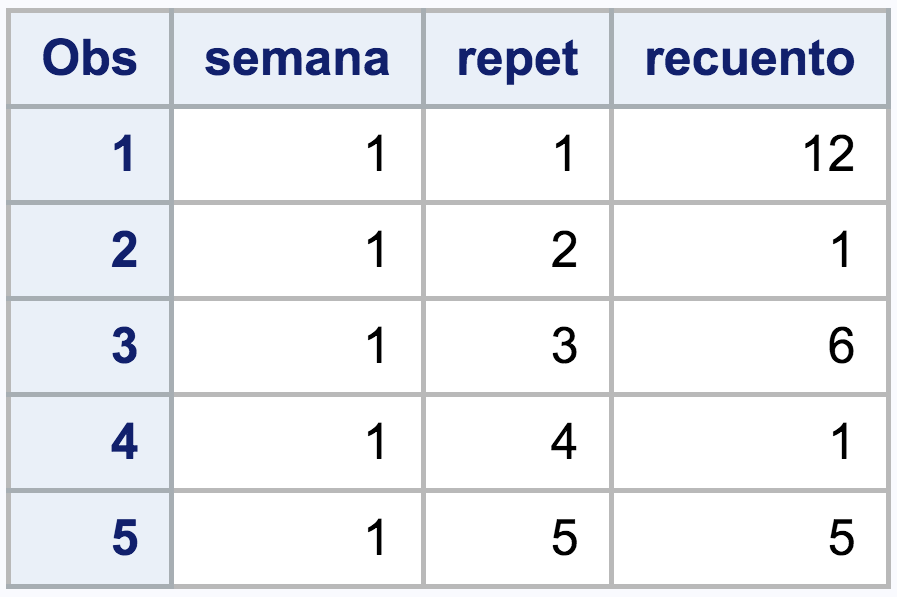
\includegraphics[width=0.3\textwidth]{pulgones-print}
      \caption{Visión preliminar del conjunto de datos \texttt{pulgones}}
      \label{img:pulgones-print}
    \end{figure}

  \section{Cuestiones}
  \label{sec:questions}

    \paragraph{}
    El objetivo general del estudio es el siguiente: \textbf{\say{Se trata de analizar si existen diferencias en el número de pulgones por planta entre las diferentes semanas}}, para lo cual se proponen una seria de sub-objetivos que se tratarán de responder en las siguientes secciones.

    \subsection{?`Es adecuado utilizar un modelo de un factor para ello? Haz un análisis descriptivo de los datos por semanas y valora las hipótesis que se asumen en el modelo.}
    \label{sec:e1}

      \paragraph{}
      Para poder responder a la pregunta sobre si es adecuado utilizar un modelo de un factor para la comparación del número de pulgones por planta entre las distintas semananas, es necesario plantearse cómo han sido recogidas las observaciones, así como estudiar si la distribución entre las distintas semanas sigue una serie temporal.

      \paragraph{}
      En el primer caso, se presupone que las $40$ observaciones referidas a cada semana han sido elegidas siguiendo algún procedimiento aleatorio. Por tanto, supondremos como válidas las observaciones para la realización del análisis de un factor.

      \paragraph{}
      En el caso de la hipótesis de que el conjunto de datos sigue un modelo de serie temporal, debe ser rechazada debido a que el contexto sobre el cual se describe el conjunto de datos no especifica que se trate distribución temporal. Esto se debe a que se indica que las plantas sobre las que se realizan las observaciones son seleccionadas en cada semana, es decir, no se sigue la evolución de las plantas durante las semanas. Además, tampoco se indica que el identificador de las semanas se refiera al orden temporal. Por tanto, debido a que no se han indicado dichas afirmaciones sobre el carácter del conjunto de datos (y el objetivo de este trabajo no es el de realizar un estudio desde el punto de vista de serie temporal del conjunto de datos), se presupondrá que las semanas se refieren a distintos factores del número de pulgones.

      \paragraph{}
      [TODO ]


    \subsection{Realiza el contraste de igualdad de medias y analiza los residuos. ?`Qué conclusiones sacas?}
    \label{sec:e2}

      \paragraph{}
      [TODO ]


    \subsection{Realiza el test de \emph{Levene}. ?`Te sorprende el resultado?}
    \label{sec:e3}

      \paragraph{}
      [TODO ]


    \subsection{Transforma la respuesta mediante $log(recuento + 1)$ y repite el apartado \ref{sec:e2}. ?`Qué cambios observas?}
    \label{sec:e4}

      \paragraph{}
      [TODO ]


    \subsection{Realiza el test de \emph{kruskal-Wallis} sobre los datos originales para contrastar la igualdad de medias}
    \label{sec:e5}
      \paragraph{}
      [TODO ]

  \section{Código fuente}
  \label{sec:code}

    \begin{figure}
      \centering
      \begin{minted}[frame=single,framesep=5pt]{sas}
data pulgones;
  do semana=1 to 6;
    do repet=1 to 40;
      input recuento @@;
      output;
    end;
  end;
  datalines;
  12 1 6 1 5 7 1 1 2 1 20 0 9 7 0 12 2 0 0 2 8 0 11 2 21 0 3 18 2 2 6 6
  5 1 12 0 3 1 1 18 40 16 32 15 44 41 43 53 67 21 6 31 15 11 21 40 15 50
  17 32 24 7 25 11 64 22 50 27 3 46 45 10 8 27 34 19 86 83 17 36 86 63
  20 68 55 42 24 29 20 27 26 63 40 46 7 15 10 30 46 26 15 42 6 28 7 9 5
  35 6 9 108 38 35 64 21 20 62 25 0 0 29 2 3 0 4 2 6 7 5 4 6 0 0 5 1 3 2
  2 2 5 0 1 1 0 3 1 2 0 3 3 18 7 21 0 0 0 2 3 0 40 5 7 0 0 0 1 1 2 1 0
  25 1 0 0 0 0 0 0 0 5 0 2 0 0 0 2 0 0 0 4 0 0 0 0 2 0 0 0 0 2 1 0 0 1 7
  0 0 0 4 1 5 2 0 0 0 0 0 0 0 0 0 0 0 0 0 0 0 0 0 0 0 0 0 0 0 0 0 0 0 0
;
run;
      \end{minted}
      \caption{\emph{Código SAS:} Lectura del conjunto de datos}
      \label{code:sas_1}
    \end{figure}


    \begin{figure}
      \centering
      \begin{minted}[frame=single,framesep=5pt]{sas}
proc print data=pulgones (obs=5) n;
run;
      \end{minted}
      \caption{\emph{Código SAS:} Vista preliminar del conjunto de datos}
      \label{code:sas_2}
    \end{figure}

    %-----------------------------
    %	Bibliographic references
    %-----------------------------

    \nocite{rano2017}

    \bibliographystyle{acm}
    \bibliography{bib}

\end{document}
